\documentclass{article}

\usepackage{amsmath, mathtools, amsthm}

\usepackage{graphicx}
\graphicspath{ {./images/automi} }

\title{Automi}
\author{github.com/asdrubalini}
\date{\today}

\begin{document}
    \maketitle

    Automa: software generico che può funzionare su qualsiasi dispositivo programmabile.
    Un automa può essere progettato graficamente con l'utilizzo di due simboli: freccia e cerchio.
    Una volta che la progettazione è conclusa, l'automa deve essere programmato con un vero e proprio linguaggio di programmazione.

    \begin{center}
        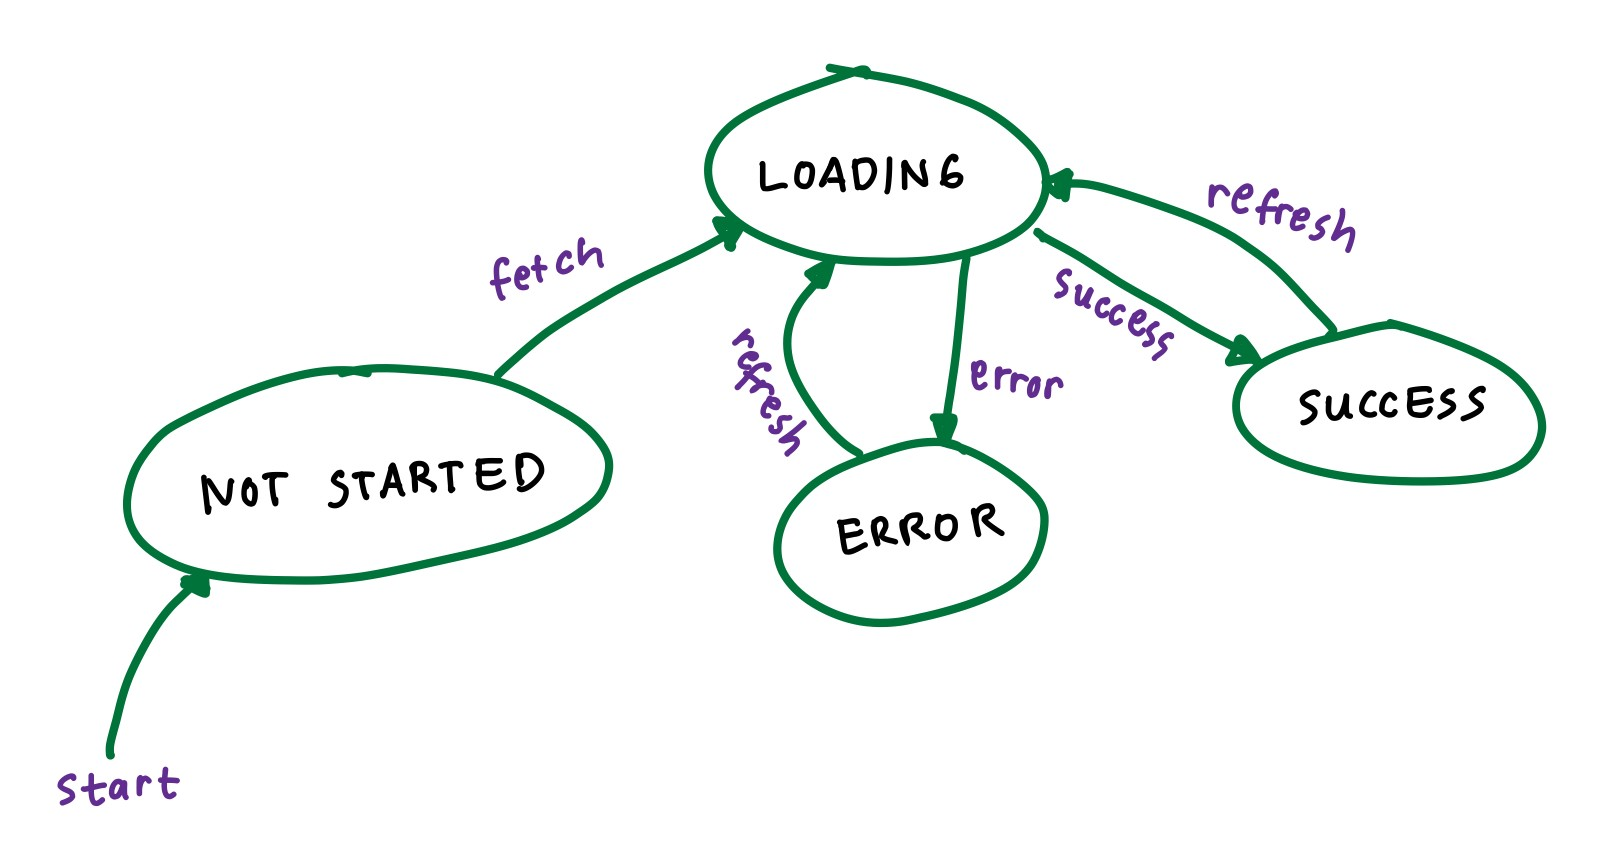
\includegraphics[width=\textwidth]{automa.png}
        esempio di diagramma che descrive un'automa
    \end{center}

    Lo stato del sistema può mutare grazie ad un evento che può essere interno (un timer) o esterno (la pressione di un bottone).
    Lo stato di partenza è essenziale, e coincide con lo stato che viene eseguito dopo l'attivazione del programma.

    \newpage

    Esercitazione: progettare l'automa che fa funzionare un semaforo.
    Verde e rosso devono avere la stessa durata (30s) mentre l'arancione deve avere un quarto della durata (7.5s). 

    \begin{center}
        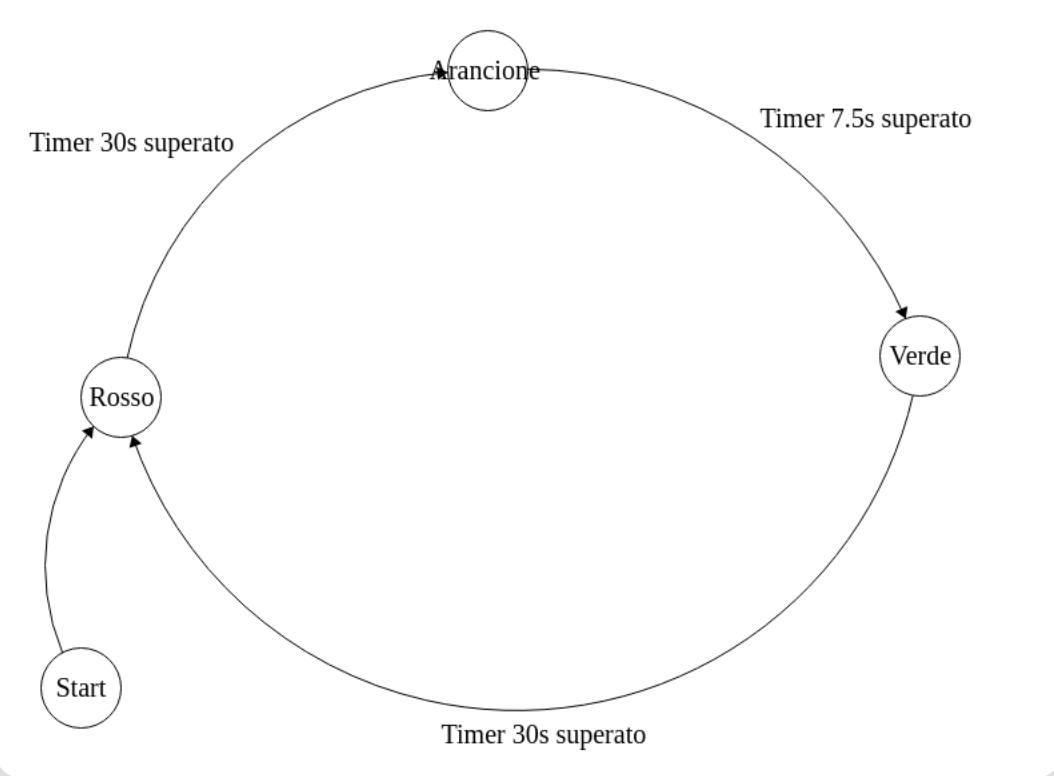
\includegraphics[width=\textwidth]{semaforo.png}
    \end{center}

    PLC: Programmable Logic Controller
    \newline
    Nati per risolvere in modo automatico reti elettriche e automi elettromeccanici.
    \newline
    Da un punto di vista elettronico sono reti combinatorie e automi con flip flop.

    Oggi i TLC sono connessi in rete ma non è necessario che sia così. Originariamente i PLC venivano programmati in un linguaggio
    particolare chiamato KOP o Ladder che si basa sulle porte logiche, interruttori e bobine.

    DSP permettono di eseguire azioni in tempi rapidissimi.

\end{document}
